\documentclass[11pt,a4paper]{article}

\usepackage[utf8]{inputenc}
\usepackage[T1]{fontenc}
\usepackage{lmodern}
\usepackage[french]{babel}
\usepackage[margin=2.1cm]{geometry}
\usepackage{microtype}
\usepackage{amsmath,amssymb}
\usepackage{booktabs}
\usepackage{array}
\usepackage[table]{xcolor}
\usepackage{graphicx}
\usepackage{caption}
\usepackage[most]{tcolorbox}

\definecolor{navy}{HTML}{1F3864}
\definecolor{bluemid}{HTML}{2E5496}
\definecolor{lightblue}{HTML}{D6E0F0}

\captionsetup{font=small,labelfont={bf,color=navy},labelsep=period}
\graphicspath{{../figures/}}

\newtcolorbox{cle}[1][]{colback=lightblue!40,colframe=navy,boxrule=0.6pt,
  arc=2pt,left=8pt,right=8pt,top=6pt,bottom=6pt,#1}

\title{\vspace{-1.2cm}\color{navy}\bfseries Des KPI descriptifs aux KPI pilotables\\[2pt]
  \large Attribution de l'écart de capital DORA, canal par canal}
\author{Kélian Kaddouri}
\date{27 juillet 2026}

\begin{document}
\maketitle
\vspace{-0.9cm}

\begin{cle}
\textbf{Approfondir les KPI.} Les cas d'usage (08e/08f/08g) et le script~39 ont produit des KPI
\emph{observables}~: délai de notification (P2), durée de confinement (P3), concentration tiers
(P4), fréquence d'entrée. Ils \textbf{décrivent} le risque. Cette note les rend
\textbf{pilotables}~: chacun est rattaché à un canal du moteur de capital, et l'on mesure le
\textbf{capital en jeu} derrière ce KPI, c'est-à-dire l'écart de SCR entre l'état conforme
(cible DORA) et l'état non conforme. On obtient un tableau de bord de remédiation.
\end{cle}

\medskip
\noindent\textbf{Quatre KPI, quatre canaux} (états conforme $\to$ non conforme déjà dans le
modèle, scripts 16/38/39)~: fréquence $\to\lambda$ ($21{,}6 \to 53{,}6$/an), détection P2/P3
$\to p_u$ ($\times 0{,}85 \to \times 1{,}20$), propagation $\to g$ ($0{,}45 \to 0{,}90$, le
canal $W$ non identifié), accumulation P4 $\to$ choc commun $\varphi_{cs}$ ($0 \to \gamma =
0{,}68$). On isole chaque canal, les autres restant conformes.

\medskip
\begin{center}
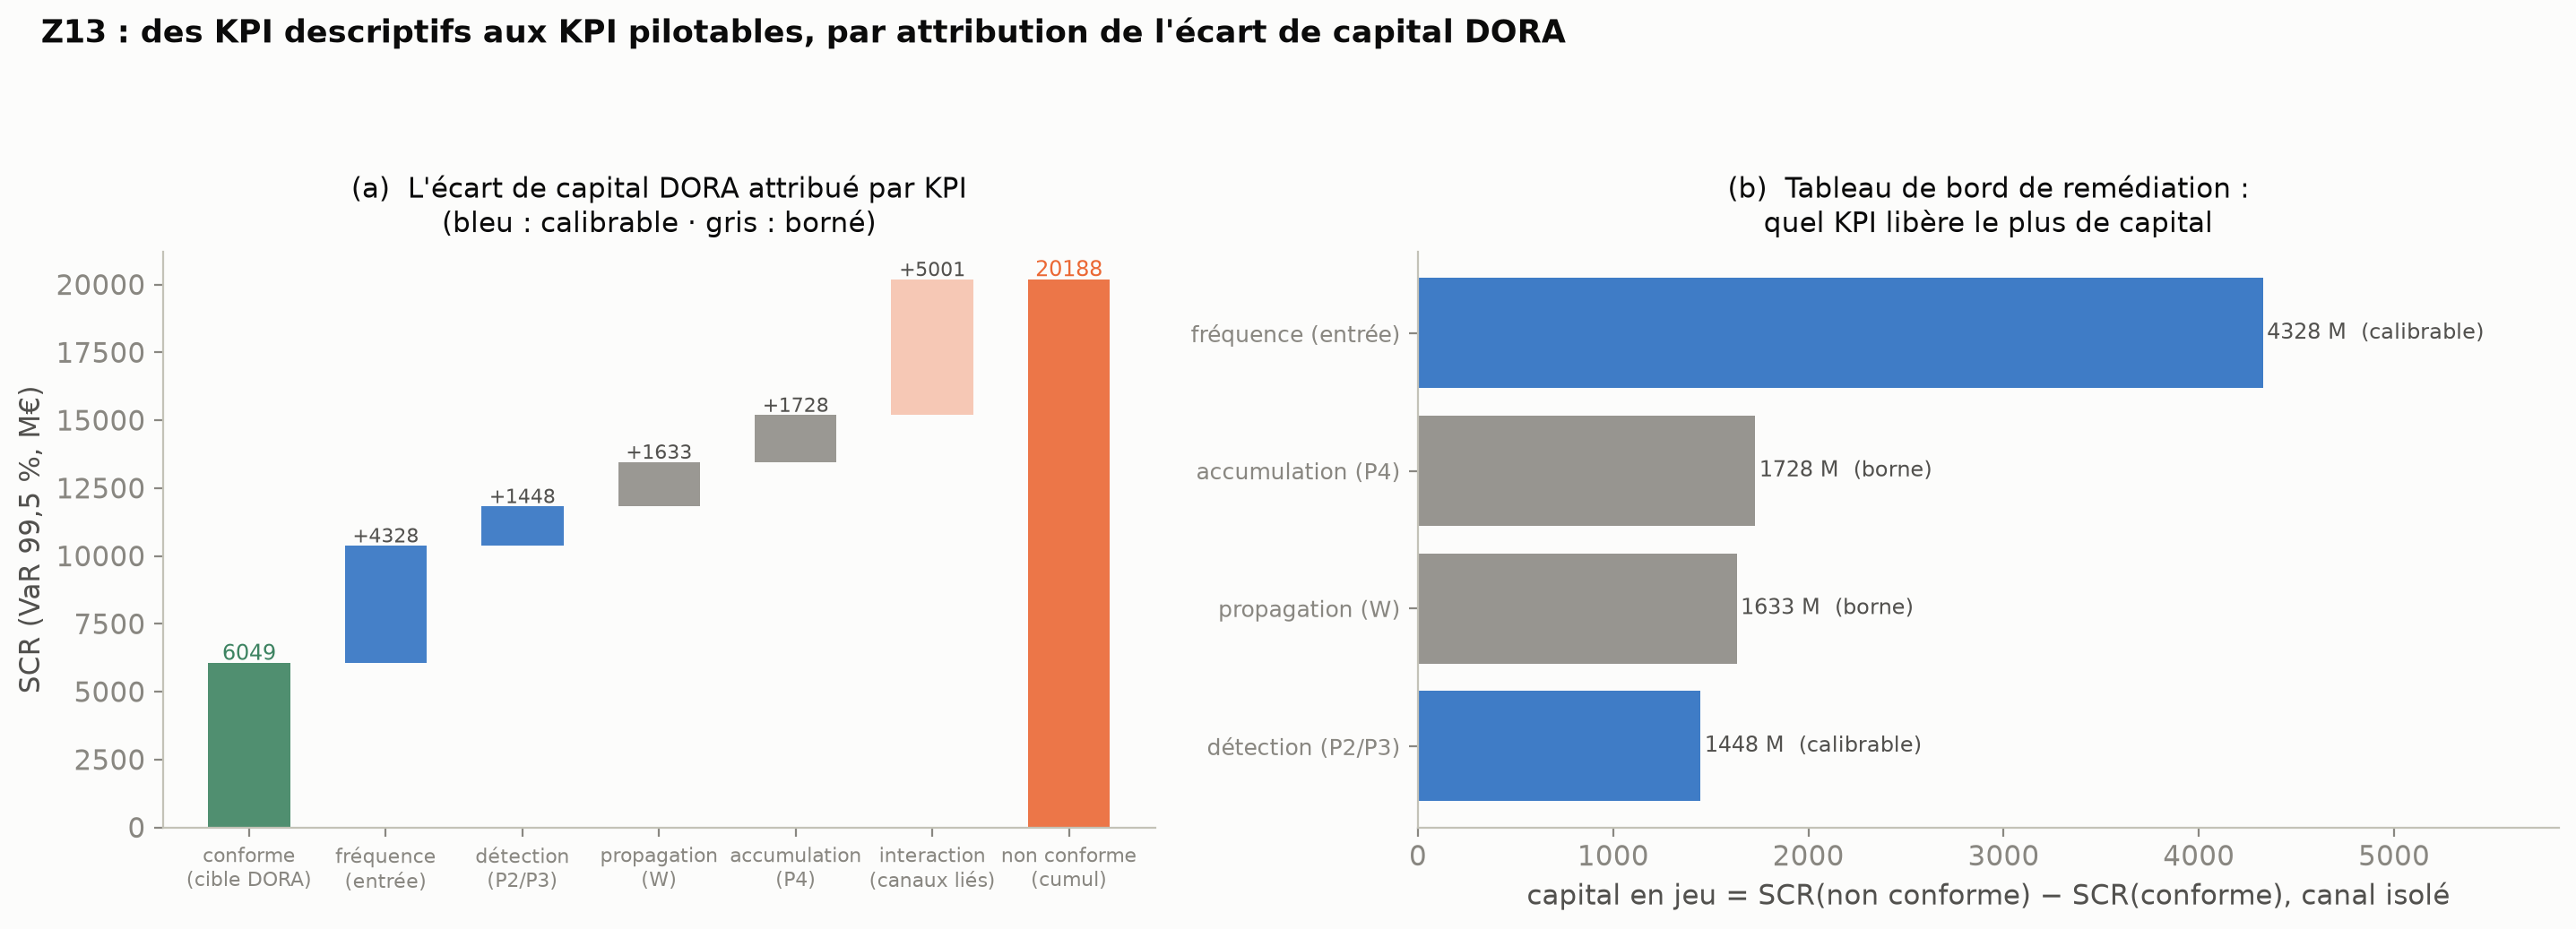
\includegraphics[width=\linewidth]{Z13_kpi_pilotables.png}
\captionof{figure}{\textbf{(a)} l'écart de capital DORA ($6\,049 \to 20\,188$ M€) attribué par
KPI, chaque canal isolé (bleu~: calibrable~; gris~: borné). Les canaux ne sont pas additifs~:
l'interaction vaut $+5\,001$ M€. \textbf{(b)} tableau de bord de remédiation~: les KPI classés
par capital libéré, avec leur statut.}
\end{center}

\begin{center}
\small
\renewcommand{\arraystretch}{1.15}
\begin{tabular}{@{}l r l l@{}}
\toprule
\textbf{KPI / canal} & \textbf{Capital en jeu} & \textbf{Statut} & \textbf{Lecture} \\
\midrule
Fréquence d'entrée (08b)          & $4\,328$ M€ & calibrable & levier actionnable \\
Accumulation P4 (concentration)   & $1\,728$ M€ & borné      & à résorber par la donnée \\
Propagation $W$                   & $1\,633$ M€ & borné      & non identifié (registre DORA) \\
Détection P2/P3                   & $1\,448$ M€ & calibrable & levier actionnable \\
\midrule
\textit{Interaction (canaux liés)} & $+5\,001$ M€ & --- & non-additivité \\
\bottomrule
\end{tabular}
\captionof{table}{Écart de capital DORA total $14\,139$ M€ (OpRisk). Somme des canaux isolés
$9\,138$ M€~; l'interaction ($+35\,\%$) traduit l'amplification par non-conformité simultanée.}
\end{center}

\begin{cle}
\textbf{Le message actionnable.} On classe les KPI par capital en jeu \textbf{et} par statut.
Les KPI à fort capital et \textbf{calibrables} (fréquence, détection) sont les leviers de
remédiation à activer en priorité. Ceux à fort capital mais \textbf{bornés} (propagation,
accumulation) disent surtout l'incertitude~: on les résorbe par la donnée (registre DORA),
pas par une action directe. Distinguer les deux est le point. C'est l'aval du fil du mémoire~:
la même discipline conforme\,/\,non conforme, bande, identification, exprimée cette fois en KPI
opposables à un souscripteur ou à un superviseur.
\end{cle}

\smallskip
\noindent\footnotesize\textcolor{navy}{\textbf{Source.}} Script
\texttt{9\_cas\_usage/43\_kpi\_pilotables.py}, figure \texttt{Z13\_kpi\_pilotables.png}.
Généralise le script~39 (canal détection) aux quatre canaux. Réutilise le harnais de choc
commun du script~38.

\end{document}
